\documentclass[10pt]{article}

\usepackage[margin=0.72in]{geometry}
\usepackage{amsmath}
\usepackage{booktabs}
\usepackage{etoolbox}
\usepackage{graphicx}
\usepackage{microtype}
\usepackage{tabularx}
\usepackage{xcolor}
\usepackage[colorlinks=true,allcolors=blue!55!black]{hyperref}

\graphicspath{{../docs/research/figures/}}
\newcommand{\shohin}{\textsc{Shohin}}
\newcommand{\pp}{\,pp}
\newcommand{\best}[1]{\textbf{#1}}
\apptocmd{\thebibliography}{\setlength{\itemsep}{0pt}\setlength{\parskip}{0pt}}{}{}

\title{\shohin: Learned Temporal Ownership for\\
Model-Owned Drafting, Revision, and Commitment}
\author{Anonymous Authors}
\date{Evidence snapshot: August 19, 2026}

\begin{document}
\maketitle

\begin{abstract}
Can distinct learned owners for drafting, revision, and commitment convert an
executed multi-stage inference budget into additional task accuracy?
\shohin{} tests this question without a test-time external verifier or answer-level
ensemble. On a protected 538-problem board, a dense Qwen3.5-9B
draft$\rightarrow$revision$\rightarrow$whole-trajectory-commit system solves
383 problems versus 316 for a matched unchanged second pass. Trained revision
also produces positive aggregate gains across five dense hosts spanning
0.8B--9B parameters and three families. Moving to sparse hosts, a
32,784-parameter incremental temporal gate reaches 143/256 on
Qwen3.6-35B-A3B, versus 111 for a source-only host and 141 for the
draft-matched trained-revision branch. A 1.66M-parameter GPT-OSS-120B
revision reaches 111/256, versus 101 source-only and 103 self-refinement. On
non-Qwen Mixtral-8x22B, a
3.54M-parameter revision surface scores 448/1,023 and beats draft-matched
self-refinement by 92 answers, while exposing severe code and source-only-case
retention regressions. The evidence supports parameter-efficient model-owned
revision across three sparse families, but not a monotonic MoE scaling law or
universal improvement: sparse commitment is untested, and the measured
auxiliary selector is not conservative.
\end{abstract}

\section{Introduction}

Inference-time computation improves language-model performance when it is
allocated through search, sampling, or adaptive refinement
\cite{wang2022selfconsistency,snell2024testtime}. These approaches raise a
structural question: must extra compute be organized by an external verifier
or answer aggregator, or can a model learn internally differentiated temporal
roles that make later computation more capable than an unchanged second pass?

We study a simple hypothesis. A first model state should own a complete draft;
a separately trained state should own full-trajectory revision; and a learned
commitment mechanism should conservatively choose one coherent answer. This
differs from asking the same model to ``try again.'' Prompted self-refinement
can improve outputs \cite{madaan2023selfrefine}, but intrinsic self-correction
can also regress reasoning \cite{huang2024selfcorrect}. We therefore compare
learned revision to both an unchanged second pass and matched self-refinement
on the same identities. Dense comparisons match both controls on the
model-owned draft and output budget; sparse comparisons use a source-only host
as the unchanged baseline and self-refinement as the draft-matched control.

Our main result is a protected dense 9B release that solves 383/538 problems,
compared with 316/538 for unchanged and 374/538 for trained revision alone.
The effect is not isolated to one checkpoint: aggregate revision gains repeat
across Qwen3.5-0.8B, 4B, and 9B, SmolLM3-3B, and OLMo2-7B. We then test whether
the temporal principle transfers to sparse models without training their
native routers or experts. A draft-conditioned gated system is strongest on a
35B-total Qwen MoE screen; trained post-MoE revision improves both controls on
117B-total GPT-OSS and produces a large replicated gain on 141B-total Mixtral.

The negative results are as important as the gains. Mixtral revision loses
executable-code capability and retains only 64.6\% of source-only-correct
validation identities. An external selector restores code and 93.2\%
retention but gives back much of the gain; model-owned sparse commitment is
untested. This separates capability acquisition from preservation of
already-correct behavior.

\paragraph{Contributions.}
\begin{enumerate}
  \item A model-owned temporal architecture with separately learned draft,
        revision, and coherent commitment roles.
  \item A protected 9B end-to-end capability result with immutable model,
        adapter, runtime, and result identities.
  \item Aggregate revision transfer across five dense hosts and three model
        families.
  \item Positive trained-revision gains across Qwen 35B, GPT-OSS 117B, and
        Mixtral 141B MoE screens, while keeping native sparse routers and
        experts frozen.
  \item A measured capability--retention boundary that exposes the need for a
        future model-owned sparse commitment mechanism.
\end{enumerate}

\section{Architecture}

Let $G(\theta,p;b)$ denote bounded generation by state $\theta$ from prompt
$p$ with output budget $b$. The dense lifecycle first produces
\begin{equation}
  d = G(\theta+\delta_{\mathrm{draft}},x;b),
\end{equation}
then a complete revision
\begin{equation}
  r = G(\theta+\delta_{\mathrm{revision}},x\Vert d;b).
\end{equation}
In the dense lifecycle, a matched unchanged role produces a complete
trajectory $u$ from the same source and draft under the same budget. The
commit owner emits one member of $\{u,r\}$; it cannot average logits or splice
answer fragments. In the sparse experiments below, unchanged is instead a
source-only host baseline; self-refinement is the draft-matched prompt control.

For a frozen feed-forward or MoE block $m_l$ at layer $l$, the transferable
Mixtral revision surface is
\begin{equation}
  m'_l(h)=m_l(h)+\frac{\alpha}{q}B_lA_lh,
  \label{eq:residual}
\end{equation}
where $q$ is residual rank. Only $A_l$ and $B_l$ are trained. The executed
Mixtral transfer controls the final 16 layers, uses $q=18$ and $\alpha=18$,
and trains 3,538,944 parameters. Native routers, experts, attention,
embeddings, and the language-model head remain frozen.

The Qwen causal gate freezes learned owner and revision residual branches and
trains only
\begin{align}
  g_l(h) &= \sigma(w_lh+b_l),\\
  m'_l(h) &= m_l(h)+\Delta_{o,l}(h)
  +g_l(h)\left[\Delta_{r,l}(h)-\Delta_{o,l}(h)\right].
  \label{eq:gate}
\end{align}
Thus $g_l=0$ recovers owner behavior and $g_l=1$ recovers revision behavior.
The reported gate adds 32,784 trainable parameters atop two frozen
1,179,648-parameter residual branches (2,392,080 \shohin{} parameters total)
and uses response loss only, with no selector target or auxiliary routing label.

\begin{figure*}[t]
  \centering
  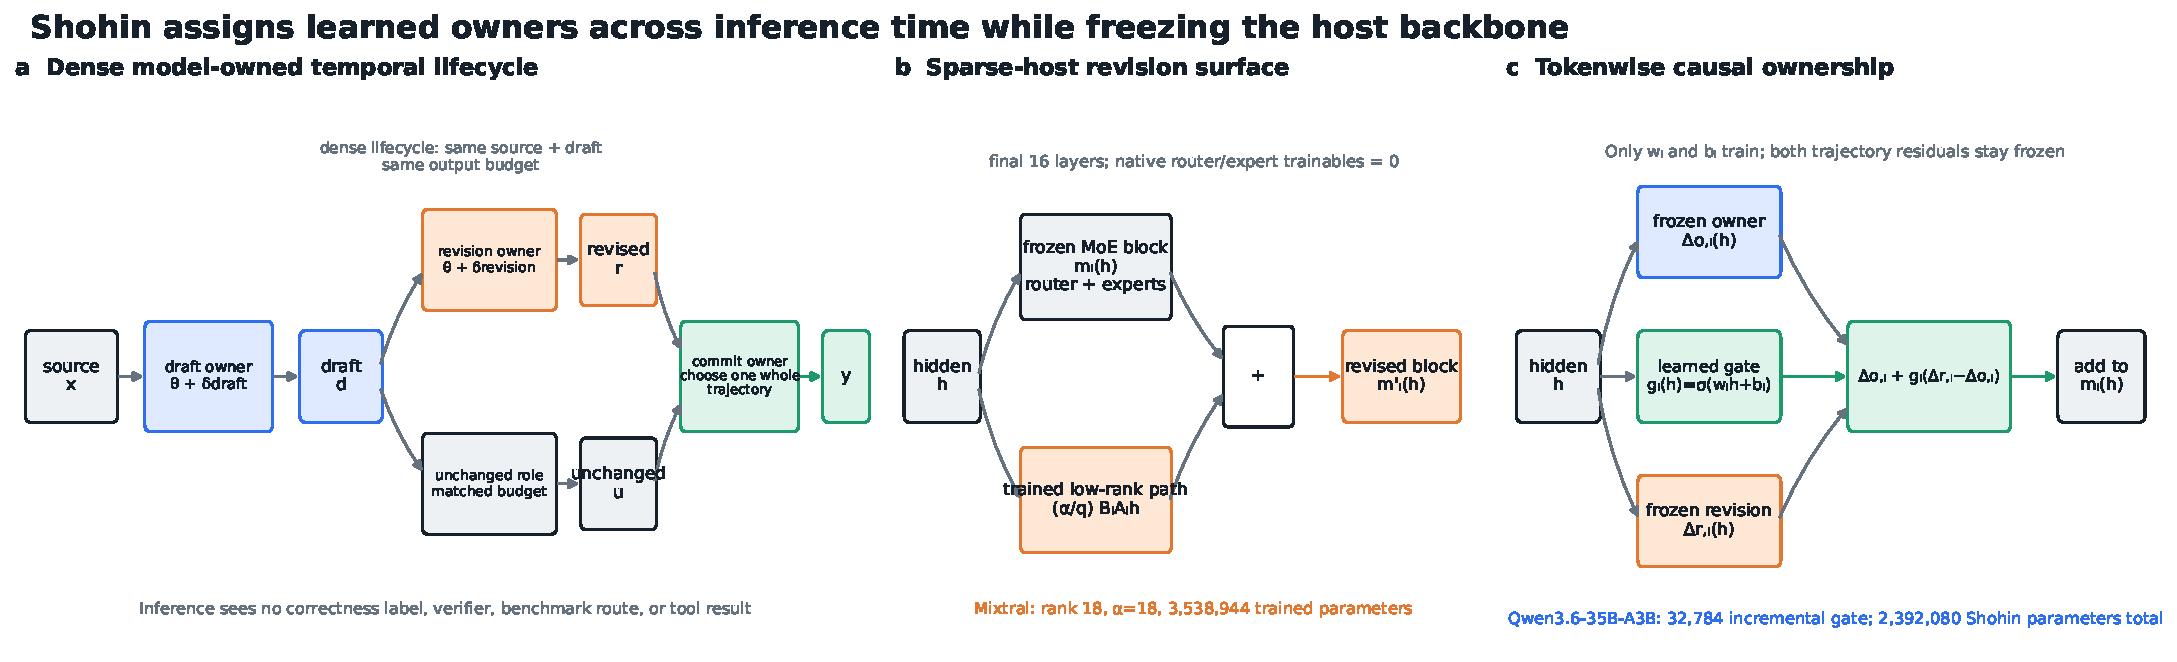
\includegraphics[width=\textwidth]{shohin_temporal_revision_architecture.pdf}
  \caption{\textbf{Learned ownership across inference time.} (a) A model-owned
  draft feeds matched unchanged and trained-revision roles; commitment selects
  one whole trajectory. (b) The sparse-host revision surface augments the final
  frozen MoE blocks. (c) The causal gate interpolates frozen owner and revision
  residuals token by token.}
  \label{fig:architecture}
\end{figure*}

\section{Experimental design}

Every capability comparison holds evaluation identities and decoding fixed.
Self-refinement receives the same draft as trained revision but uses a fixed
natural-language correction instruction. Dense unchanged also receives that
draft; sparse unchanged is source-only. Thus sparse revision-versus-unchanged
measures the full draft-conditioned pipeline against the host, while
revision-versus-self-refinement isolates learned revision under matched draft
access. Source-disjoint screens and holdouts are identity-separated from
training inputs. Protected boards remain outside model-visible training and
generation paths.

All gains are paired on exact identities. When available, we report discordant
win/loss counts and exact two-sided McNemar tests. Parameter counts include only
trained \shohin{} surfaces. Predeclared retention and per-domain gates remain
binding even when aggregate accuracy improves, so a large numerical gain can
still be a non-promotion.

The primary protected board contains GSM8K (100), MATH-500 (100), executable
code (40), GPQA (198), and BBH logic (100), for 538 scored identities. The dense
transfer boards contain 1,289 development or 1,279 holdout identities drawn
from mathematics, logic/science, and execution-verified code. The MoE screens
use a fixed source-disjoint 256-row board; Mixtral validation uses 1,023
independent rows (497 logic, 504 mathematics, 22 code).

\section{Results}

\subsection{Protected dense release}

\begin{table}[h]
\centering
\small
\caption{Protected Qwen3.5-9B result. Macro averages the five main domains;
AIME is diagnostic and excluded from the 538 denominator.}
\begin{tabular}{lrrrr}
\toprule
System & Solved & Macro & Code & AIME\\
\midrule
Unchanged second pass & 316/538 & 67.263\% & 34/40 & 4/30\\
Trained revision & 374/538 & 75.005\% & 35/40 & 3/30\\
Learned commit & \best{383/538} & \best{75.815\%} & 35/40 & 6/30\\
Coherent oracle (not deployable) & 399/538 & 78.619\% & 35/40 & 6/30\\
\bottomrule
\end{tabular}
\label{tab:protected}
\end{table}

The learned commit adds 67 solved problems over unchanged and nine over trained
revision. An independently parameterized commit control solves 382/538, so the
supported claim is useful learned coherent commitment, not a unique advantage
of one antisymmetric scoring parameterization. Candidate-order consistency is
100\% with zero swap error. Three prompt truncations in the product application
are disclosed rather than silently recoded.

\subsection{Dense transfer}

\begin{table}[h]
\centering
\small
\caption{Trained revision versus matched unchanged. H and D denote holdout and
development evidence.}
\begin{tabular}{lrrl}
\toprule
Host & Split & Correct (revision / unchanged) & Delta\\
\midrule
Qwen3.5-0.8B & H & 328 / 242 & +6.72\pp\\
Qwen3.5-4B & H & 554 / 380 & +13.60\pp\\
Qwen3.5-9B & H & 625 / 495 & +10.16\pp\\
SmolLM3-3B & D & 469 / 358 & +8.61\pp\\
OLMo2-7B & D & 259 / 231 & +2.17\pp\\
\bottomrule
\end{tabular}
\label{tab:dense}
\end{table}

All five hosts improve in aggregate, but the table does not imply monotonic
per-domain transfer. Qwen0.8B and SmolLM3 regress executable code; OLMo2 is too
weak to promote; and the Qwen4 protected board fails its all-domain criterion.

\subsection{Gated Qwen MoE transfer}

On Qwen3.6-35B-A3B (35B total, 3B active), the temporal gate scores 143/256
versus 111/256 for the source-only host: +32 answers / +12.5\pp, with 38 paired
wins and six losses ($p=9.43\times10^{-7}$). This comparison measures the full
draft-conditioned gated system, not the gate alone. Against the draft-matched
trained-revision branch (141/256), the gate adds two answers (three wins, one
loss; $p=.625$). It retains 105/111 source-only-correct identities. Mean
revision weight rises from 0.643 at the first controlled layer to 0.903 at the
last; these layer means describe the learned routing profile but do not by
themselves exclude a fixed layer-specific gate.

\subsection{GPT-OSS-120B transfer}

Pinned GPT-OSS-120B has 117B total and 5.1B active parameters. A
1,658,880-parameter post-MLP revision surface controls the final 16 layers
while native MXFP4 router and expert tensors remain frozen. On the same
source-disjoint 256-row screen used for the other MoE points:

\begin{table}[h]
\centering
\small
\caption{GPT-OSS-120B matched screen.}
\begin{tabular}{lrrrr}
\toprule
Arm & Correct & Logic & Math & Code\\
\midrule
Unchanged (source-only) & 101 & 78 & 12 & 11\\
Self-refinement & 103 & 81 & 11 & 11\\
Trained revision & \best{111} & \best{82} & \best{18} & 11\\
\bottomrule
\end{tabular}
\label{tab:gptoss}
\end{table}

Revision adds ten answers over source-only (19 wins / 9 losses,
$p=.0872$) and eight over draft-matched self-refinement (12 / 4,
$p=.0768$). Logic improves by four, mathematics by six, and all 11 MBPP
solutions are preserved relative to source-only. The result nevertheless
fails the frozen conservative boundary: only 92/101 (91.09\%) source-only-
correct identities remain correct. Mechanics, training, 12 independent
one-H100 evaluation allocations, and CPU scoring complete with zero retries;
charged usage is 26,322 H100-seconds (7.3117 H100-hours).

\subsection{Cross-family Mixtral transfer}

Mixtral-8x22B has 141B total and 39B active parameters. Its revision surface is
0.00251\% of total and 0.00907\% of active parameters. Both draft-conditioned
arms use the same immutable Qwen3.6-35B-A3B drafts, making this a deliberately
cross-family model-owned transfer.

\begin{table}[h]
\centering
\small
\caption{Mixtral validation on 1,023 identities.}
\begin{tabular}{lrrrr}
\toprule
Arm & Correct & Logic & Math & Code\\
\midrule
Unchanged (source-only) & 147 & 106 & 25 & 16\\
Self-refinement & 356 & 224 & 121 & 11\\
Trained revision & \best{448} & \best{272} & \best{176} & 0\\
Auxiliary selector & 287 & 222 & 49 & \best{16}\\
\bottomrule
\end{tabular}
\label{tab:mixtral}
\end{table}

Revision gains 301 answers over the source-only host and 92 over the clean,
draft-matched self-refinement control. The paired comparisons are 353 wins /
52 losses versus the source-only host ($p=4.44\times10^{-56}$) and 131 / 39
versus self-refinement ($p=7.92\times10^{-13}$). The 256-row screen shows the
same ordering: 114 revision, 105 self-refinement, and 45 source-only.

The result is not a qualified universal release. Revision retains only 95/147
(64.6\%) source-only-correct validation identities and loses all 22 code rows.
A task-label-free three-way auxiliary linear selector restores 16/22 code and
improves all domains over source-only, but scores only 287 and retains 137/147
(93.2\%), three cases below the frozen 95\% floor. It uses hashed source and
completion features, including strong output-modality proxies, and is trained
on per-arm correctness labels from the 256-row screen without task identity;
it is not the in-model two-way commit used by the dense release. Its formal
gate fails.

An identity-joined replay of all 1,023 scored candidate triples shows that the
code failure is systematic (Table~\ref{tab:format}).

\begin{table}[h]
\centering
\small
\caption{Measured Mixtral output-form collapse. Boxed is over all 1,023 rows;
the final three columns are over 22 MBPP rows.}
\begin{tabular}{lrrrrr}
\toprule
Arm & Mean tokens & Boxed & Fences & Definitions & Code correct\\
\midrule
Unchanged & 436.13 & 203 & 22 & 21 & 16\\
Self-refinement & 296.84 & 454 & 22 & 19 & 11\\
Trained revision & 9.99 & 1,023 & 0 & 0 & 0\\
\bottomrule
\end{tabular}
\label{tab:format}
\end{table}

Revision's median output is nine tokens overall and seven on MBPP; no code
completion contains a return statement. The scorer requires explicit final
answer form on answer-valued tasks, so the measured gain includes successful
answer-format transfer and does not by itself isolate better reasoning. The
surface violates executable output modality. The auxiliary selector restores
code by selecting unmodified trajectories, localizing the next architecture
problem to model-owned output-contract preservation. Without receiving a task
label, the selector chooses unchanged for all 22 MBPP
identities and restores 16 correct programs. Yet it also selects unchanged for
460/504 mathematics identities and the stronger revision only 10 times. It can
therefore recognize overt output modality, but not yet promote scored
answer-valued gains while preserving that modality.

\begin{figure*}[t]
  \centering
  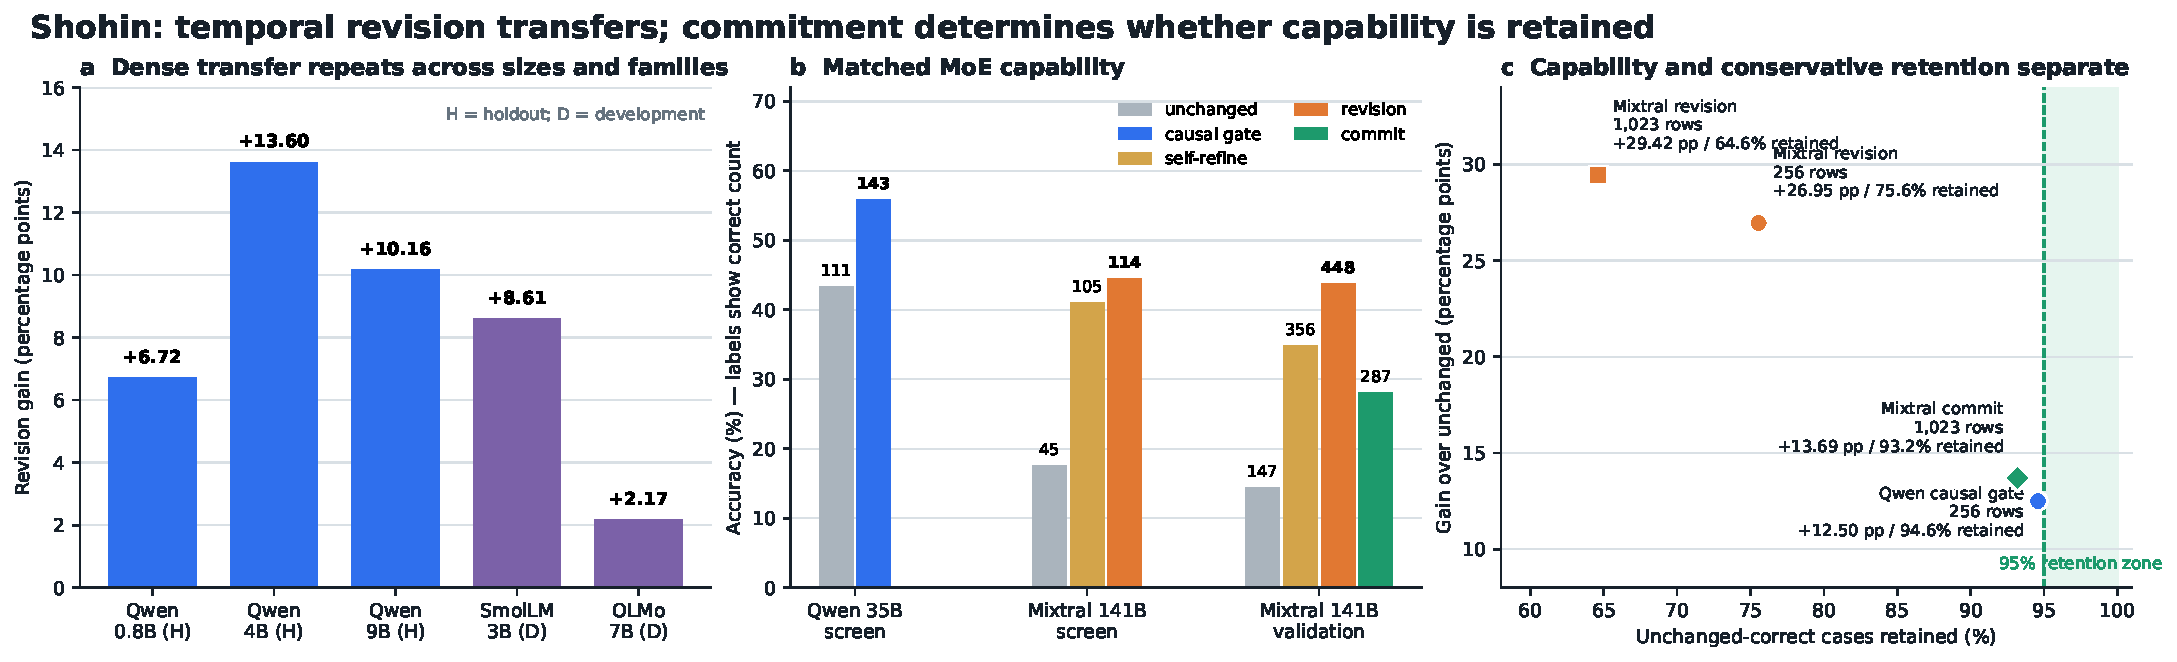
\includegraphics[width=\textwidth]{shohin_temporal_revision_evidence.pdf}
  \caption{\textbf{Capability transfer and its retention boundary.} Dense
  gains repeat across sizes and families. Sparse bars label source-only and
  draft-conditioned arms explicitly. Retention is measured against source-only;
  capability delta is measured against each draft-matched comparator.}
  \label{fig:evidence}
\end{figure*}

\section{Discussion}

Three observations survive the full evidence boundary. First, learned temporal
revision consistently exceeds matched dense unchanged roles and beats both
sparse controls on all three completed MoE-family screens. Sparse gains over
source-only hosts additionally include access to the frozen draft. Second, the
GPT-OSS and Mixtral gains require no trainable native routing or expert
parameters; the Qwen gate is the strongest measured Qwen system but adds only
two answers over its frozen trained-revision branch. Third, capability and
retention are distinct optimization targets. Revision finds new correct
trajectories but can overwrite already-correct behavior. The external
auxiliary selector restores some conservatism but not the full large-host gain;
model-owned sparse commitment has not yet been measured.

The three MoE screens do not support a monotonic scaling law. Qwen 35B,
GPT-OSS 117B, and Mixtral 141B each show positive revision gains over both
controls, but gain is nonmonotonic by active parameters, retention misses 95\%
at multiple points, and Mixtral code regresses. A weighted active-parameter
slope is positive under an independent marginal sampling approximation, while
the total-parameter interval crosses zero; three heterogeneous points are
insufficient for a general scaling claim. Nemotron Super failed before science
and Ultra has not run; neither is evidence.

\section{Related work}

Self-Refine \cite{madaan2023selfrefine} and Reflexion
\cite{shinn2023reflexion} use textual feedback or reflection. \shohin{} makes
self-refinement a matched control and learns a separate revision role. LoRA
\cite{hu2021lora} and ReFT \cite{wu2024reft} motivate parameter-efficient
weight and representation interventions; our residual surfaces add an explicit
temporal contract and are evaluated with model-owned prior trajectories.

Switch Transformers \cite{fedus2021switch} route tokens among experts, while
Mixture-of-Depths \cite{raposo2024mod} routes tokens across layer compute.
Recurrent-depth latent reasoning \cite{geiping2025recurrent} and Coconut
\cite{hao2024coconut} extend internal computation without requiring every step
to be natural language. \shohin{} tests a complementary axis: which learned
temporal state should own a token or a complete answer after a draft already
exists.

\section{Limitations and reproducibility}

The primary protected result is one pinned 9B host and should not be read as a
universal theorem. Dense aggregate gains include domain failures. The Qwen MoE
evidence is a 256-row development screen, and its source-only comparison does
not isolate draft access from learned routing. GPT-OSS is also a 256-row
screen; its positive paired differences do not reach $p<.05$ and its
retention gate fails. Mixtral validates at 1,023 rows
but fails conservative retention and code; its scorer rewards required answer
form, and no format-agnostic replay is claimed. The multi-stage systems also
use more generation calls and tokens than a single unchanged pass, so these
results are not compute-normalized. Public leaderboard superiority and a
monotonic MoE scaling law are not supported.

All headline artifacts bind exact model revisions, trainable checkpoints,
runtime manifests, source identities, arm outputs, and score reports. The
protected 9B product report SHA-256 is
\texttt{3e86751b...f7187}; the Qwen MoE screen is
\texttt{1bd64551...b4871}; the GPT-OSS raw score is
\texttt{906b3b01...d59}; the Mixtral validation raw score is
\texttt{7befd864...c3d8}. Full hashes and the complete result ledger are in the
companion evidence report. Both figures are deterministically generated by
\path{pipeline/render_shohin_publication_figure.py}.

\begingroup
\scriptsize
\bibliographystyle{plain}
\bibliography{references}
\endgroup

\end{document}
